\documentclass{beamer}
\usepackage{HECbeamer}
\usepackage{icomma}
% \usepackage{pgfpages}
% \pgfpagesuselayout{4 on 1}[letterpaper, landscape, border shrink=5mm]
\title[\color{white}{MATH 60604 \S~4e - Tableaux de contigence}]{\texorpdfstring{MATH 60604 \\Modélisation statistique \\ \S~4e - Tableaux de contigence}{MATH 60604 \\Modélisation statistique \\ \S~4e - Tableaux de contigence}}
\author{}
\institute{HEC Montréal\\
Département de sciences de la décision}
\date{} 

\begin{document}
\frame{\titlepage}
\begin{frame}[fragile]
 \frametitle{Tableaux de contingence bidimensionnels}
 Le format le plus commun pour les données de dénombrement sont les \textbf{tableaux de contingence}, dans lesquels les dimensions sont les modalités des variables catégorielles et les cellules le décompte par sous-catégorie.
 
 Soit $\mathrm{X}_1$ et $\mathrm{X}_2$ deux variables catégorielles avec respectivement $J$ et $K$ niveaux. Le nombre d'événement pour chaque sous-catégorie est représenté à l'aide du tableau de contingence
 \begin{center}
  \begin{tabular}{c|cccc}
   &$\mathrm{X}_2=1$ & $\mathrm{X}_2=2$ & $\cdots$ & $\mathrm{X}_2=K$\\\specialrule{\cmidrulewidth}{0pt}{0pt}
   $\mathrm{X}_1=1$ & $Y_{11}$ & $Y_{12}$ & $\cdots$ & $Y_{1K}$ \\
   $\mathrm{X}_1=2$ & $Y_{21}$ & $Y_{22}$ & $\cdots$ & $Y_{2K}$ \\
  $\vdots$  & $\vdots$ & $\ddots$  & $\ddots$ &  $\vdots$ \\
  $\mathrm{X}_1=J$ & $Y_{J1}$ & $Y_{J2}$ & $\cdots$ & $Y_{JK}$
 \end{tabular}
\end{center}

\end{frame}
\begin{frame}[fragile]
\frametitle{Test d'indépendance dans un tableau de contingence}

\bi \item On considère deux modèles de Poisson: sous $\Hy_0$, le modèle avec les deux variables explicatives catégorielles, mais \textbf{sans interaction}. Pour $(j= 1, \ldots, J; k=1, \ldots, K)$, le nombre moyen dans la cellule $(j,k)$
 \begin{align*}
  \mu_{jk} = \exp\left(\beta_0 + \alpha_j \I{\mathrm{X}_{1}=j} + \gamma_k \I{\mathrm{X}_{2}=k}\right).
 \end{align*}
où $\alpha_1=0$ et $\gamma_1=0$ pour des raisons d'identifiabilité des paramètres. 
\item 
Le modèle sous l'alternative est le modèle saturé qui inclut en plus une interaction entre $\mathrm{X}_1$ et $\mathrm{X}_2$.
L'hypothèse nulle d'indépendance revient à tester si les paramètres additionnels pour l'interaction sont zéros.

\ei 
\end{frame}
\begin{frame}
 \frametitle{Modèle saturé et modèle avec effets principaux pour tableaux de contingence}
 \bi \item Sous $\Hy_0$, le modèle inclut seulement $\mathrm{X}_1$ et $\mathrm{X}_2$ (effets principaux). 
  \bi 
  \item On peut montrer que la valeur ajustée de ce modèle nul est simplement le produit des proportions par ligne/colonne. 
  \item On dénote la valeur ajustée pour la cellule $(j,k)$ par $\hat{\mu}_{jk}$.
  \ei
  \item Le modèle saturé, sous l'hypothèse alternative $\Hy_1$, inclut des paramètres pour l'interaction.
    \bi \item le modèle saturé a $n=JK$ paramètres et la valeur ajustée est $Y_{jk}$.
\ei 
\ei 
\end{frame}
\begin{frame}
 \frametitle{Statistiques du test d'indépendance dans les tableaux de contingence}
    \bi 
  \item La statistique du rapport de vraisemblance est la déviance 
  \begin{align*}
   D= 2 \sum_{j=1}^J \sum_{k=1}^K Y_{jk}\ln \pfrac{Y_{jk}}{\hat{\mu}_{jk}}
  \end{align*}
qui suit une loi $\chi^2_{(J-1)(K-1)}$ sous l'hypothèse nulle d'indépendance.
\item On peut également utiliser un test du score (avec la même loi asymptotique),
\begin{align*}
 X^2 = \sum_{j=1}^J \sum_{k=1}^K \frac{(Y_{jk}-\hat{\mu}_{jk})^2}{\hat{\mu}_{jk}}.
\end{align*}

  \ei 
\end{frame}
\begin{frame}[fragile]
 \frametitle{Affiliation politique aux États-Unis}
 On considère un tableau de contingence deux par trois de l'affiliation politique d'Américain(e)s en fonction de leur sexe (données de 2000).
 \begin{center}
 \begin{tabular}{llllc}
 \toprule 
  & \multicolumn{3}{c}{Affiliation} & \\
  \cmidrule(r){2-4}
  sexe & démocrate & indépendant & républicain & Total\\
  femmes & $762$ & $327$ & $468$ & $1557$ \\
   & ($703.7$) & ($319.6$) & ($533.7$) & \\
   hommes & $484$ & $239$ & $477$ & $1200$ \\
    & ($542.3)$ & $(246.4)$ & $(411.3)$ & \\
    total & $1246$ & $566$ & $945$ &$2757$\\
    \bottomrule 
    \end{tabular}
    \end{center}
    Les valeurs entre parenthèses dénotent les valeurs ajustées du modèle Poisson avec les deux variables catégorielles, mais sans interactions (effets principaux).

     
     \vp
  {   \footnotesize
 Tableau 2,5 de  Agresti (2007), \textsl{An Introduction to
Categorical Data Analysis}, Wiley.


}
\end{frame}
\begin{frame}
 \frametitle{Résultats du test d'indépendance  pour l'affiliation politique}
   \bi \item     
En ajustant le modèle sans interaction, on obtient la statistique du $X^2$ de Pearson et la déviance à même la sortie ($30.07$ et $30.02$, respectivement).
\item Si l'affiliation politique ne dépendait pas du sexe, ces statistiques devraient suivre approximativement une loi $\chi^2_2$.
\item Les valeurs-$p$ sont inférieures à $10^{-4}$ et on rejette l'indépendance; l'affiliation politique dépend du sexe de l'individu.
\ei
\begin{center}
 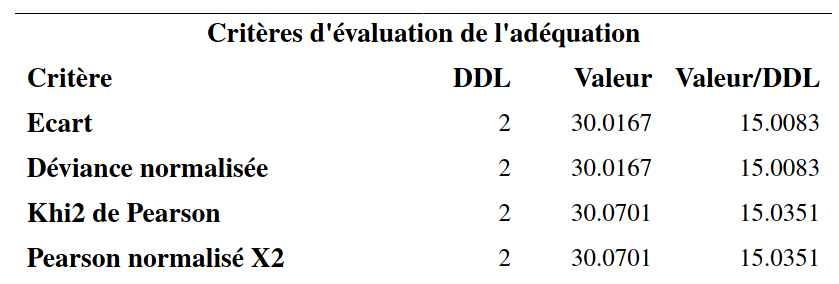
\includegraphics[width = 0.8\linewidth]{img/c4/diapos8-e1}
\end{center}
\end{frame}


\end{document}
